\clearpage

\subsection{例題6 文字に色を付けてみる}

\subsection*{考え方}

mes命令で表示する文字に色を付けるにはcolor命令を使います。

\begin{figure}[H]
    \begin{center}
        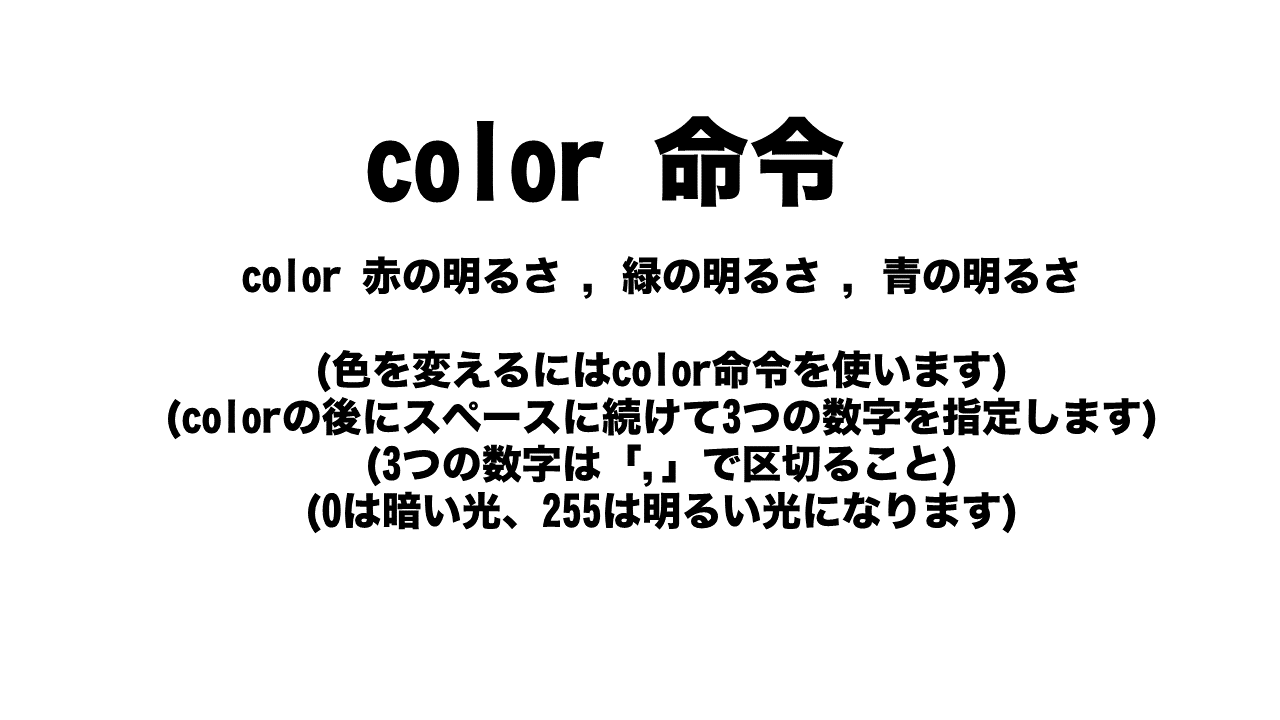
\includegraphics[keepaspectratio,width=12.277cm,height=5.08cm]{text02-img/text02-img030.png}
    \end{center}
\end{figure}

明るさとは、その成分がどのくらい明るいかということを示している\ruby{数値}{すう|ち}です。

明るさは、0がもっとも
\ruby{暗}{くら}くて、255が\ruby{最}{もっと}も\ruby{明}{あか}るい状態になります。

これらを組み合わせて、1670万以上の色を
出すことができます。この時に指定する色のことをRGBと呼んでいます。

\subsubsection*{RGBとは}

光の3原色は赤、緑、青紫ですが、赤と緑をまぜるとイエローに、緑と青紫をまぜるとシアンに、青紫と赤をまぜるとマゼンタになります。
光の3原色を等分にまぜると明るくなって、\ruby{白色光}{はく|しょく|こう}になります。これを「\ruby{加法混色}{か|ほう|こん|しょく}」といいます。
RGBカラーはテレビやモニタなどの「光り」で色を\ruby{表現}{ひょう|げん}する方式です。

\begin{figure}[H]
    \begin{center}
        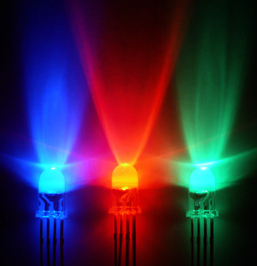
\includegraphics[keepaspectratio,width=3.854cm,height=3.988cm]{text02-img/text02-img033.jpg}
    \end{center}
\end{figure}

RGBの意味は R:レッド(赤) G:グリーン(緑) B:ブルー(青)の\ruby{頭文字}{かしら|も|じ}です。
赤・緑・青それぞれの光の強さを0から255までの数値で表わします。
黒は、赤・緑・青のどれも光らせない(強さ0)ことで表現します。
白は赤・緑・青すべてを光らせた時(強さ255)の色になります。
\clearpage
モニターで色がついているのも、すべての点で3つの色(RGB)が光っているからです。コンピューターが、それぞれの点(ドット)をせいぎょして光らせているのです。

\begin{figure}[H]
    \begin{center}
        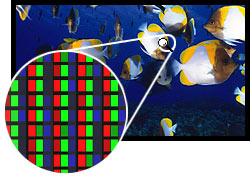
\includegraphics[keepaspectratio,width=3.854cm,height=3.988cm]{text02-img/text02-img034.jpg}
        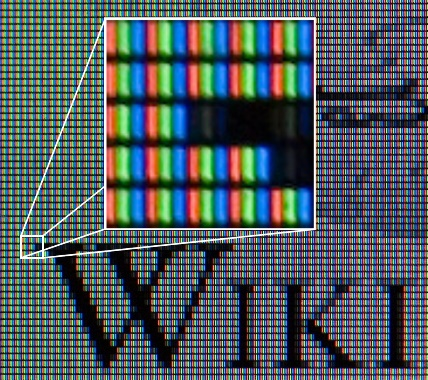
\includegraphics[keepaspectratio,width=3.854cm,height=3.988cm]{text02-img/text02-img035.jpg}
    \end{center}
\end{figure}

mes命令の前に書かれているcolor命令の数字を変更することで、「OK!」の文字に使われている色を変えることができます。
自分で色を選んで、好きな色で文字を出してみましょう。

\subparagraph*{例題6 答え}

必ず、mes命令が実行されるよりも前(上の行)にcolor命令を書きます。
代表的な色は次のようになります。参考にして思った通りの色になっているか確認してみましょう。

\begin{description}
    \item color 0 ,0 ,0 ; ← 黒 
    \item color 0 ,0 ,255 ; ← 青 
    \item color 255 ,0 ,0 ; ← 赤 
    \item color 255 ,0 ,255 ; ← 紫 
    \item color 0 ,255 ,0 ; ← 緑
    \item color 0 ,255 ,255 ; ← 水色
    \item color 255 ,255 ,0 ; ← 黄色
    \item color 255 ,255 ,255 ; ← 白
\end{description}

「; ← 黒」のように行の中で「;」が入っている部分から先は「コメント」として扱われます。
「;」から先は、命令を書いても実行の時にも\ruby{無視}{む|し}されます。
「コメント」は、その行でやっていること、残しておきたいメモなどを書くことのできる機能です。

